\documentclass[10pt,a4paper]{article}
\usepackage[utf8]{inputenc}
\usepackage[spanish]{babel}
\usepackage{amsmath}
\usepackage{textcomp}
\usepackage{amsfonts}
\usepackage{amssymb}
\usepackage{enumerate}
\usepackage{graphicx}
\usepackage[left=2cm,right=2cm,top=2cm,bottom=2cm]{geometry}
\author{Gonzalo Moreno Soto\\ Alejandro Pérez Argüello\\ Miguel Piñar Pérez\\ Gerardo Tirado García\\ Irene Trigueros Lorca\\ Alejandro Villanueva Prados}
\title{Relación 2 de EDIP.}
\begin{document}
\maketitle

\newpage
\begin{enumerate}
\item Se han lanzado 2 dados varias veces, obteniendo los resultados que se presentan en la siguiente tabla, donde X designa el resultado del primer dado e Y, el resultado del segundo:

\vspace{0.5cm}
\begin{tabular}{|c|c|c|c|c|c|c|c|c|c|c|c|c|c|c|c|c|c|c|c|c|c|c|c|c|}
\hline 
X & 1 & 2 & 2 & 3 & 5 & 4 & 1 & 3 & 3 & 4 & 1 & 2 & 5 & 4 & 3 & 4 & 4 & 5 & 3 & 1 & 6 & 5 & 4 & 6 \\ 
\hline 
Y & 2 & 3 & 1 & 4 & 3 & 2 & 6 & 4 & 1 & 6 & 6 & 5 & 1 & 2 & 5 & 1 & 1 & 2 & 6 & 6 & 2 & 1 & 2 & 5 \\ 
\hline 
\end{tabular} 

\vspace{0.5cm}
\hspace{0.25cm} a) Construir la tabla de frecuencias.

\vspace{0.5cm}
\begin{tabular}{|c|c|c|c|c|c|c|c|c|c|}
\hline 
X  \textbackslash  Y & 1 & 2 & 3 & 4 & 5 & 6 & $n_{i\cdot}$ & $x_in_{i\cdot}$ & $(x_i- \bar{x})^2n_{i\cdot}$ \\ 
\hline 
1 & 0 & 1 & 0 & 0 & 0 & 3 & 4 & 4 & 361/16 \\ 
\hline 
2 & 1 & 0 & 1 & 0 & 1 & 0 & 3 & 6 & 363/64 \\ 
\hline 
3 & 1 & 0 & 0 & 2 & 1 & 1 & 5 & 15 & 45/64 \\ 
\hline 
4 & 2 & 3 & 0 & 0 & 0 & 1 & 6 & 24 & 75/32 \\ 
\hline 
5 & 2 & 1 & 1 & 0 & 0 & 0 & 4 & 20 & 169/16 \\ 
\hline 
6 & 0 & 1 & 0 & 0 & 1 & 0 & 2 & 12 & 441/32 \\ 
\hline 
$n_{\cdot j}$ & 6 & 6 & 2 & 2 & 3 & 5 & 24 & 81 & 6043/32 \\ 
\hline 
$y_jn_{\cdot j}$ & 7 & 10 & 6 & 8 & 15 & 30 & 76 &  &  \\ 
\hline 
$(y_j-\bar{y})^2n_{\cdot j}$ & 2809/36 & 841/96 & 25/288 & 361/288 & 1849/192 & 22445/576 & 87.6929  &   &   \\ 
\hline 
\end{tabular} 

\vspace{0.5cm}
\hspace{0.25cm} b) Calcular las puntuaciones medias obtenidas de cada dado y ver cuáles son más homogéneas.

\vspace{0.5cm}
\begin{equation*}
\bar{y} = \dfrac{\displaystyle\sum_{j = 1}^6(y_{i}*n_{\cdot j})}{N} = \frac{77}{24} \simeq 3.208333 \simeq 3 \textrm{ puntos}
\end{equation*}

\begin{equation*}
\bar{x} = \dfrac{\displaystyle\sum_{i = 1}^6(x_{i}*n_{\cdot i})}{N} = \frac{81}{24} \simeq 3.375 \simeq 3 \textrm{ puntos} 
\end{equation*}

\begin{equation*}
\sigma_y = \sqrt{\displaystyle\sum_{j = 1}^6 \dfrac{(y_j - \bar{y})^2 n_j}{N}} = \sqrt{\dfrac{87.6929}{24}} = 1.91151
\end{equation*}

\begin{equation*}
\sigma_x = \sqrt{\displaystyle\sum_{i = 1}^6 \dfrac{(x_i - \bar{x})^2 n_i}{N}} = \sqrt{\dfrac{6043}{32*24}} = 2.80508
\end{equation*}

Las puntuaciones obtenidas por el dado Y son más homogéneas.

\vspace{0.5cm}
\hspace{0.25cm} c) ¿Qué resultado del 2º dado es más frecuente cuando en el 1º se obtiene un 3?

El 4

\vspace{0.5cm}
\hspace{0.25cm} d) Calcular la puntuación máxima del 50\% de las puntuaciones más bajas obtenidas con el primer dado si con el segundo se ha obtenido un 2 o un 5?

\vspace{0.25cm}

\begin{tabular}{|c|c|c|c|c|}
\hline 
  & (4,2) & (5,2) = (2,5) & (6,2) = (3,5) & (6,5) \\ 
\hline 
$z_i$ & 6 & 7 & 8 & 11 \\ 
\hline 
$n_i$ & 3 & 2 & 2 & 1 \\ 
\hline 
$N_i$ & 3 & 5 & 7 & 8 \\ 
\hline 
\end{tabular}

\vspace{0.25cm}
Mediana: $\dfrac{N}{2} = 4 \Rightarrow $ Me = 7

\newpage
\item Medidos los pesos, X (en kg) y las alturas (en cm) Y, a un grupo de individuos se han obtenido los siguientes resultados:

\vspace{0.5cm}
\begin{tabular}{|c|c|c|c|c|c|c|c|c|c|}
\hline 
X \textbackslash Y & 160 & 162 & 164 & 166 & 168 & 170 & $n_{i\cdot}$ & $x_in_{i\cdot}$ & $(x_i - \bar{x})^2 n_{i\cdot}$ \\ 
\hline 
48 & 3 & 2 & 2 & 1 & 0 & 0 & 8 & 384 & 304.6922 \\ 
\hline 
51 & 2 & 3 & 4 & 2 & 2 & 1 & 14 & 714 & 140.8114 \\ 
\hline 
54 & 1 & 3 & 6 & 8 & 5 & 1 & 24 & 1296 & 0.7053 \\ 
\hline 
57 & 0 & 0 & 1 & 2 & 8 & 3 & 14 & 798 & 112.0114 \\ 
\hline 
60 & 0 & 0 & 0 & 2 & 4 & 4 & 10 & 600 & 339.72245 \\ 
\hline 
$n_{\cdot j}$ & 6 & 8 & 13 & 15 & 19 & 9 & 70 & 3792 & 897.84275 \\ 
\hline 
$y_jn_{\cdot j}$ & 960 & 1296 & 2132 & 2490 & 3192 & 1530 & 11600 &   &   \\ 
\hline 
$(y_j - \bar{y})^2 n_{\cdot j}$ & 9600/49 & 5408/49 & 1872/49 & 60/49 & 4864/49 & 8100/49 & 4272/7 &   &   \\ 
\hline 
\end{tabular}

\vspace{0.5cm}
\hspace{0.25cm} a) Calcular el peso medio y la altura media y decir cuál es más representativo.

\begin{equation*}
\bar{y} = \dfrac{\displaystyle\sum_{j = 1}^6(y_{i}*n_{\cdot j})}{N} = \frac{11600}{70} \simeq 165.7143 \simeq 166 \textrm{ cm}
\end{equation*}

\begin{equation*}
\sigma_y^2 = \displaystyle\sum_{j = 1}^6 \dfrac{(y_j - \bar{y})^2 n_{\cdot j}}{N} = \dfrac{2136}{245} \simeq 8.7184 \textrm{ cm}^2
\end{equation*}

\begin{equation*}
\sigma_y = \sqrt{\sigma_y^2} = 2.952688156
\end{equation*}

\begin{equation*}
C.V.P.(y) = \dfrac{\sigma_y}{\bar{y}} = 0.0178179
\end{equation*}

\begin{equation*}
\bar{x} = \dfrac{\displaystyle\sum_{i = 1}^6(x_{i}*n_{\cdot i})}{N} = \frac{3792}{70} \simeq 54.1714 \simeq 54 \textrm{ kg} 
\end{equation*}

\begin{equation*}
\sigma_x^2 = \displaystyle\sum_{i = 1}^5 \dfrac{(x_i - \bar{x})^2 n_{i \cdot}}{N} = \dfrac{897.94275}{70} \simeq 12.82775 \textrm{ kg}^2
\end{equation*}

\begin{equation*}
\sigma_x = \sqrt{\sigma_x^2} = 3.581585
\end{equation*}

\begin{equation*}
C.V.P.(x) = \dfrac{\sigma_x}{\bar{x}} = 0.0661158
\end{equation*}

\vspace{0.25cm} La media de la altura es más representativa, ya que el coeficiente de variación de Pearson de Y es menor.

\vspace{0.5cm}
\hspace{0.25cm} b) Calcular el porcentaje de individuos que pesan menos de 55 kg y miden más de 165 cm.

\vspace{0.5cm}
Tal y como se presentan las variables en la tabla, la altura y el peso son variables discretas, por lo que el número de individuos que pesan menos de 55 kg son los que pesan menos o igual a 54 kg; los que miden más de 165 cm son los que miden más o igual a 166 cm.

\begin{equation*}
\displaystyle\sum_{i=1}^{3} \displaystyle\sum_{j=4}^{6} \dfrac{n_{ij}}{N} * 100 = \dfrac{1+2+8+2+5+1+1}{70} * 100 = 28.5714 \%
\end{equation*}

\vspace{0.5cm}
\hspace{0.25cm} c) Entre los que miden más de 165 cm, ¿cuál es el porcentaje de los que pesan más de 52 kg?

Número de personas que miden más de 165 cm: 70 - 27 = 43

\begin{equation*}
\displaystyle\sum_{i=3}^{5} \displaystyle\sum_{j=4}^{6} \dfrac{n_{ij}}{43} * 100 = \dfrac{8+5+1+2+8+3+2+4+4}{43} * 100 = 86.0465 \%
\end{equation*}

\vspace{0.5cm}
\hspace{0.25cm} d) ¿Cuál es la altura más frecuente entre los individuos cuyo peso oscila entre 51 y 57 kg?

\vspace{0.5cm}
La altura más frecuente entre los individuos que pesan entre 51 kg y 57 kg es 168 cm.

\vspace{0.5cm}
\hspace{0.25cm} e) ¿Qué peso medio es más representativo el de los individuos que miden 164 cm o el de los que miden 168 cm?

\vspace{0.5cm}
\begin{equation*}
\bar{x}_{y = 164 \textrm{ cm}} = \dfrac{\displaystyle\sum_{i = 1}^5(x_{i}*n_{\cdot i})}{N} = \frac{2*48 + 4*51 + 6*54 + 1*57}{13} = \dfrac{681}{13} \textrm{ kg} = 52.3846 \textrm{ kg} 
\end{equation*}

\begin{equation*}
\sigma_{x_{y = 164 \textrm{ cm}}}^2 = \displaystyle\sum_{i = 1}^5 \dfrac{(x_i - \bar{x})^2 n_{i \cdot}}{N} = \dfrac{1080}{169} \simeq 6.3905 \textrm{ kg}^2
\end{equation*}

\begin{equation*}
\sigma_{x_{y = 164 \textrm{ cm}}} = \sqrt{\sigma_{x_{y = 164 \textrm{ cm}}}^2} = \dfrac{6 \sqrt{30}}{13}
\end{equation*}

\begin{equation*}
C.V.P.(x_{y = 164 \textrm{ cm}}) = \dfrac{\sigma_{x_{y = 164 \textrm{ cm}}}}{\bar{x}_{y = 164 \textrm{ cm}}} = 0.0482575
\end{equation*}

\begin{equation*}
\bar{x}_{y = 168 \textrm{ cm}} = \dfrac{\displaystyle\sum_{i = 1}^5(x_{i}*n_{\cdot i})}{N} = \frac{2*51 + 5*54 + 8*57 + 4*60}{19} = \dfrac{1086}{19} \textrm{ kg} = 56.2105 \textrm{ kg} 
\end{equation*}

\begin{equation*}
\sigma_{x_{y = 168 \textrm{ cm}}}^2 = \displaystyle\sum_{i = 1}^5 \dfrac{(x_i - \bar{x})^2 n_{i \cdot}}{N} = \dfrac{2682}{361} \simeq 7.4294 \textrm{ kg}^2
\end{equation*}

\begin{equation*}
\sigma_{x_{y = 168 \textrm{ cm}}} = \sqrt{\sigma_{x_{y = 168 \textrm{ cm}}}^2} = \dfrac{3 \sqrt{298}}{19}
\end{equation*}

\begin{equation*}
C.V.P.(x_{y = 168 \textrm{ cm}}) = \dfrac{\sigma_{x_{y = 168 \textrm{ cm}}}}{\bar{x}_{y = 168 \textrm{ cm}}} = 0.047687
\end{equation*}

La media más representativa es la de los individuos de 168 cm.
\newpage

\item En una encuesta de familias sobre el número de individuos que la componen ($X$) y el número de personas activas en ellas ($Y$) se han obtenido los siguientes resultados:

\begin{center}
\begin{tabular}{c|cccc}
$X \backslash Y$ & 1 & 2 & 3 & 4 \\\hline
1 & 7 & 0 & 0 & 0 \\
2 & 10 & 2 & 0 & 0 \\
3 & 11 & 5 & 1 & 0 \\
4 & 10 & 6 & 6 & 0 \\
5 & 8 & 6 & 4 & 2 \\
6 & 1 & 2 & 3 & 1 \\
7 & 1 & 0 & 0 & 1 \\
8 & 0 & 0 & 1 & 1 \\
\end{tabular}
\end{center}

\begin{itemize}
\item[a)]Calcular la recta de regresión de $Y$ sobe $X$.

$y=0,3147x + 0,5322$.

\item[b)]¿Es adecuado suponer una relación lineal para explicar el comportamiento de $Y$ a partir de $X$?

Según el coeficiente de correlación lineal $$r = \frac{\sigma_{xy}}{\sigma_x\sigma_y} = 0,535$$ el ajuste no es el idóneo, pero los hay peores.

\end{itemize}

\newpage

		\item Se realiza un estudio sobre la tensión de vapor de agua ($Y$, en ml. de Hg.) a distintas temperaturas($X$, en \textcelsius{}). Efectuadas 21 medidas, los resultados son:

\begin{center}
\begin{tabular}{c|ccc}
$X \backslash Y$ & (0.5, 1.5] & (1.5,2.5] & (2.5,5.5]\\\hline
(1, 15] & 1 & 2 & 0 \\
(15, 25] & 1 & 4 & 2 \\
(25, 30] & 0 & 3 & 5 \\
\end{tabular}
\end{center}

Explicar el comportamiento de la tensión de vapor en términos de la temperatura mediante una función lineal. ¿Es adecuado asumir este tipo de relación?

La recta de regresión es $$y = 0,0935x + 0,608.$$

En principio sí, porque se supone que a mayor temperatura habrá mayor evaporación.
Según el coeficiente de correlación lineal $$r = \frac{\sigma_{xy}}{\sigma_x\sigma_y} = 0,6565$$ el ajuste es más o menos adecuado, pero los hay mejores.

\newpage

\item Estudiar la dependencia o independencia de las variables en cada una de las siguientes distribuciones. Dar, en cada caso, las curvas de regresión y la covarianza de las dos variables.

\begin{center}
\begin{tabular}{c|ccccc|c}
$X \backslash Y$ & 1 & 2 & 3 & 4 & 5 & $n_{i\cdot}$\\\hline
10 & 2 & 4 & 6 & 10 & 8 & 30\\
20 & 1 & 2 & 3 & 5 & 4 & 15\\
30 & 3 & 6 & 9 & 15 & 12 & 45\\
40 & 4 & 8 & 12 & 20 & 16 & 60\\\hline
$n_{\cdot j}$ & 10 & 20 & 30 & 50 & 40 & 150\\
\end{tabular}
\end{center}

Se aprecia que 

$$n_{ij} = \frac{n_{i\cdot}\cdot n_{\cdot j}}{n} \quad \forall j = 1,2,3,4,5 \quad \forall i = 1,2,3,4$$ 

por lo que son independientes.

Por ser independientes, la covarianza es nula: $$\sigma_{xy} = 0.$$

No tiene sentido en este caso hacer la recta y la curva de regresión. Aunque la recta de regresión sería $$y = 3,6$$ la curva de regresión de $X$ sobre $Y$ sería $$(29, 1), (29, 2), (29, 3), (29, 4), (29, 5)$$ y la curva de regresión de Y sobre X sería $$(10, 3.6), (20, 3.6), (30, 3.6), (40, 3.6), (50,3.6).$$

\bigskip

\begin{center}
\begin{tabular}{c|ccc|c}
$X \backslash Y$ & 1 & 2 & 3 & $n_{i\cdot}$\\\hline
-1 & 0 & 1 & 0 & 1 \\
0 & 1 & 0 & 1 & 2 \\
1 & 0 & 1 & 0 & 1 \\\hline
$n_{\cdot j}$ & 1 & 2 & 1 & 4 \\
\end{tabular}
\end{center}

En la segunda fila y en la segunda columna hay dos frecuencias no nulas, por lo que no hay dependencia funcional.

También, se aprecia que $$n_{11} = 0 \not = \frac{n_{1\cdot}\cdot n_{\cdot 1}}{n} = \frac{1}{4},$$ por lo que no son independientes.

$$m_{10} = \bar x = 0$$
$$m_{01} = \bar y = 2$$
$$m_{11} = 0$$
$$\sigma_{xy} = m_{11} - m_{10}m_{01} = 0$$

La covarianza es nula.

Podemos considerar una recta de regresión como $$y = 2.$$

La curva de regresión de $X$ sobre $Y$ es $$(0,1), (0,2), (0,3).$$

La curva de regresión de $Y$ sobre $X$ es $$(-1,2), (0,2), (1,2).$$

\newpage

\item Dada la siguiente distribución bidimensional:

\begin{center}
\begin{tabular}{c|cccc|c}
$X \backslash Y$ & 1 & 2 & 3 & 4 & $n_{i\cdot}$\\\hline
10 & 1 & 3 & 0 & 0 & 4 \\
12 & 0 & 1 & 4 & 3 & 8 \\
14 & 2 & 0 & 0 & 2 & 4 \\
16 & 4 & 0 & 0 & 0 & 4\\\hline
$n_{\cdot j}$ & 7 & 4 & 4 & 5 & 20\\
\end{tabular}
\end{center}

\begin{itemize}

\item[a)]¿Son estadísticamente independientes X e Y?

Se aprecia que $$n_{21} = 0 \not = \frac{n_{2\cdot}\cdot n_{\cdot 1}}{n} = \frac{56}{20},$$ por lo que no son independientes.

\item[b)]Calcular y representar las curvas de regresión de $X/Y$ e $Y/X$.

La curva de regresión de $Y$ sobre $X$ es $$(10,1'75), (12,3'25), (14,2'5), (16,1).$$

La curva de regresión de $X$ sobre $Y$ es  $$(14'5714,1), (10'5,2), (12,3), (12'8,4).$$

Representación:

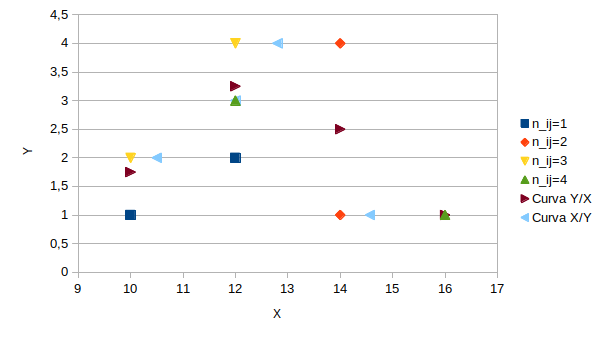
\includegraphics[width=10cm]{graficoe6.png}

\item[c)]Cuantificar el grado en que cada variable es explicada por la otra mediante la correspondiente curva de regresión.

Esto es cuantificado por la razón de correlación $\eta^2$: $$\eta^2_{Y/X} = \frac{\sigma^2_{ey}}{\sigma^2_y},$$ donde $\sigma^2_{ey}$ es la varianza explicada por la regresión $$\sigma^2_{ey} = \sigma^2_y - \sigma^2_{ry}$$ donde $\sigma^2_{ry}$ es la varianza residual $$\sigma^2_{ry} = \sum_{i=1}^k \sum_{j=1}^p f_{ij} [y_j - f(x_i)]^2$$ y $\sigma^2_y$ es la varianza de $Y$ $$\sigma^2_y = \mu_{02} = \sum_{j=1}^p f_{\cdot j}(y_j-\bar y)^2.$$
\\$\eta^2$ está entre 0 y 1; cuánto más cerca esté de 1 mejor ajustada está la correlación.

$$\bar y = 2,35$$

$$\sigma^2_y = 1,4275$$

$$\sigma^2_{ry} = 0,6625$$

$$\sigma^2_{ey} = 1,4275 - 0,6625 = 0,765$$

$$\eta^2_{Y/X} = \frac{0,765}{1,4275} = 0,5359$$

La variable $Y$ es parcialmente explicada por $X$ mediante la curva de regresión de $Y/X$.

$$\bar x = 12,8$$

$$\sigma^2_x = 4,16$$

$$\sigma^2_{ry} = 1,8757$$

$$\sigma^2_{ey} = 4,16 - 1,8757 = 2,2842$$

$$\eta^2_{X/Y} = \frac{2,2842}{4,16} = 0,5491$$

La variable $X$ es parcialmente explicada por $Y$ mediante la curva de regresión de $X/Y$.

\item[d)]¿Están $X$ e $Y$ correladas linealmente? Dar las expresiones de las rectas de regresión.

La correlación lineal se mide mediante el coeficiente de correlación lineal $r$:
$$r = \frac{\sigma_{xy}}{\sigma_x \sigma_y}$$
donde $\sigma_{xy}$ es la covarianza
$$\sigma_{xy} = \mu_{11} = m_{11} - \bar x \bar y$$
donde $m_{11}$ es el momento conjunto respecto al origen de órdenes 1 y 1,
$$m_{11} = \sum_{i=1}^k \sum_{j=1}^p f_{ij} x_i y_j,$$
$\sigma_x = +\sqrt{\sigma_x^2}$ es la desviación típica de $X$, y recíprocamente para $Y$.
\\$r$ está entre -1 y 1; cuánto más cerca esté de 0 menor es la correlación lineal.

$$m_{11} = 29,3$$
$$\sigma_{xy} = 29,3 - 12,8\cdot2,35 = -0,78$$
$$r = \frac{-0,78}{\sqrt{4,16}\sqrt{1,4275}} = -0,32008$$
La correlación lineal no explica bien la distribución.

En la recta de regresión $y = ax + b$, a es
$$a = \frac{\sigma_{xy}}{\sigma_x^2}$$
y b es
$$b = \bar y - \frac{\sigma_{xy}}{\sigma_x^2} \bar x.$$

Las expresiones de las rectas de regresión lineal son
$$y = -0,1875x + 4,75$$
y
$$x = -0,5464y + 14,08.$$

\end{itemize}

\newpage

\item Para cada una de las distribuciones:

\begin{center}
\begin{tabular}{c|ccc|c}
\multicolumn{5}{c}{Distribución A}\\
$X \backslash Y$ & 10 & 15 & 20 & $n_{i\cdot}$\\\hline
1 & 0 & 2 & 0 & 2 \\
2 & 1 & 0 & 0 & 1 \\
3 & 0 & 0 & 3 & 3 \\
4 & 0 & 1 & 0 & 1\\\hline
$n_{\cdot j}$ & 1 & 3 & 3 & 7\\
\end{tabular}
\begin{tabular}{c|ccc|c}
\multicolumn{5}{c}{Distribución B}\\
$X \backslash Y$ & 10 & 15 & 20 & $n_{i\cdot}$\\\hline
1 & 0 & 2 & 0 & 2 \\
2 & 1 & 0 & 0 & 1 \\
3 & 0 & 0 & 3 & 3 \\\hline
$n_{\cdot j}$ & 1 & 2 & 3 & 6\\

\end{tabular}
\begin{tabular}{c|cccc|c}
\multicolumn{5}{c}{Distribución C}\\
$X \backslash Y$ & 10 & 15 & 20 & 25 & $n_{i\cdot}$\\\hline
1 & 0 & 3 & 0 & 1 & 4 \\
2 & 0 & 0 & 1 & 0 & 1 \\
3 & 2 & 0 & 0 & 0 & 2 \\\hline
$n_{\cdot j}$ & 2 & 3 & 1 & 1 & 7 \\

\end{tabular}
\end{center}

\begin{itemize}

\item[a)]¿Dependen funcionalmente $X$ de $Y$ o $Y$ de $X$?

\begin{itemize}

\item[Distribución A:]$Y$ depende funcionalmente de $X$ porque para todo $x_i$ existe un único $y_j$.
\\No ocurre lo contrario, ya que para $y_2 = 15$ exiten $x_1 = 1$ y $x_4 = 4$ con frecuencias $n_{ij}$ no nulas.

\item[Distribución B:]$X$ e $Y$ tienen una dependencia funcional recíproca, ya que para todo $x_i$ existe un único $y_j$ y viceversa.
Es decir, la función que los relaciona es biyectiva.

\item[Distribución C:]$X$ depende funcionalmente de $Y$ porque para todo $y_j$ existe un único $x_i$.
\\No ocurre lo contrario, ya que para $x_1 = 1$ exiten $y_2 = 15$ y $y_4 = 25$ con frecuencias $n_{ij}$ no nulas.

\end{itemize}

\item[b)]Calcular las curvas de regresión y comentar los resultados.

\begin{itemize}

\item[Distribución A:]La curva de regresión $Y/X$ es $$(1, 15), (2, 10), (3, 20), (4, 15).$$
\\Estos puntos forman parte de la función que relaciona ambas variables, $f(X) = Y$.
\\La curva de regresión $X/Y$ es $$(2, 10), (2, 15), (3, 20).$$

\item[Distribución B:]La curva de regresión de $Y/X$ es $$(1,15), (2,10), (3,20).$$
\\La curva de regresión de $X/Y$ es $$(2,10), (1,15), (3,20).$$
\\Estas dos curvas son en realidad la misma, y forman parte de la función que asocia las variables, $g(X) = Y$ y $g^{-1}(Y) = X$.

\item[Distribución C:]La curva de regresión de $Y/X$ es $$(1, 17'5), (2, 20), (3, 10).$$
\\La curva de regresión de $X/Y$ es $$(3, 10), (1, 15), (2, 20), (1, 25).$$
\\Estos puntos forman parte de la función que relaciona ambas variables, $h(Y) = X$.

\end{itemize}

\end{itemize}

\newpage
\item
\newpage
\item
\newpage
\item
\newpage
\item
\newpage


        \item De las estadísticas de ``Tiempos de vuelo y consumos de combustible'' de una compañía aérea, se han obtenido datos relativos a 24 trayectos distintos realizados por eel avión DC-9. A partir de estos datos se han obtenido las siguientes medidas:
            \begin{center}
                \[
                \sum y_i = 219.719 \quad  \sum y_i^2 = 2396.504 \quad \sum x_i y_i = 349.486
                \]
                \[
                \sum x_i = 31.470 \quad \sum x_i^2 = 51.075 \quad \sum x_i^2 y_i = 633.993
                \]
                \[
                \sum x_i^4 = 182.977 \quad \sum x_i^3 = 93.6
                \]
            \end{center}
            La variable \(Y\) expresa el consumo total de combustible, en miles de libras, correspondiente a un vuelo de duración \(X\) (el tiempo se expresa en horas, y se utilizan como unidades de orden inferior fracciones decimales de la hora).

            \begin{enumerate}[a)]
                \item Ajustar un modelo del tipo \(Y=aX+b\). ¿Qué consumo total se estimaría para un programa de vuelos compuesto de 100 vuelos de media hora, 200 de una hora y 100 de dos horas? ¿Es fiable esta estimación?


                    \emph{Solución}: Comenzamos analizando nuestra población y los datos que tenemos: observamos que la población es de tamaño \(n=24\), además nos indican que los 24 vuelos son distintos así que \(n_i = 1; \quad \forall i \in \{1 \dots 24\}\) 


                    Una vez tomadas estas consideraciones, nos centramos en la pregunta: encontrar un ajuste lineal mediante un polinomio de grado 1. La expresión de la función será: \[y - \overline{y}=\frac{\sigma_{xy}}{\sigma_x^2}\left(x-\overline{x}\right),\] así que pasamos a calcular los datos necearios:\[\overline{x}=\frac{1}{n}\sum x_i = \frac{31.470}{24}\approx1.311\text{ Horas de vuelo},\]\[\overline{y}=\frac{1}{n}\sum y_i=\frac{219.719}{24}\approx 9.155\text{ Miles de libras de combustible},\]\[\sigma_{xy}=\frac{1}{n}\sum(x_i-\overline{x})(y_i-\overline{y})=m_{11}-m_{10}m_{01}=\frac{1}{n}\sum x_iy_i-\frac{1}{n^2}\sum x_i\sum y_i\approx 2.557\]\[\sigma_x^2=\frac{1}{n}\sum(x_i-\overline{x})^2=\frac{1}{n}\sum x_i^2 - \overline{x}^2,\approx 0.40854\] finalmente, la recta de regresión queda: \[y=6.26x+0.946.\]

                    Pasamos ahora a la segunda cuestión del apartado, para ello aplicamos la función obtenida:


                    \[ 6.26\cdot 0.5+0.946 = 4.076 \text{ (Consumo estimado para un vuelo de media hora)}\]\[6.26 \cdot 1 + 0.946 = 7.206 \text{ (Consumo estimado para un vuelo de una hora)}\]\[6.26 \cdot 2 + 0.946 = 13.466 \text{ (Consumo estimado para un vuelo de dos horas)}\] Ahora escalamos estos resultados multiplicando por el númmero de vuelos y sumamos todo, obteniendo un consumo total de \(3195.4\) miles de libras de combustible.
                    
                    Para cuantificar la fiabilidad de la predicción, vamos a emplear el coeficiente de correlación lineal, dado por \[r=\pm\sqrt{r^2}=\frac{\sigma_{xy}}{\sigma_x\sigma_y},\] calculamos \(\sigma_x\) y \(\sigma_y\): \[\sigma_x=\sqrt{\sigma_x^2}=\sqrt{0.401}\approx0.640\]\[\sigma_y=\sqrt{\frac{1}{n}\left(\sum y_i^2-\frac{1}{n}\sum y_i\right)}\approx 4.005,\] con estos datos, el coeficiente de correlación lineal queda \(0.99758\), lo que nos indica un ajuste casi perfecto y una muy alta fiabiidad.
                
                \item  Ajustar un modelo del tipo \(Y=a+bX+cX^2\). ¿Qué consumo total se estimaría para el mismo programa de vuelos del apartado a)?

                    \emph{Solución}: Los coeficientes de nuestra función de ajuste vienen dados por las soluciones del siguiente sistema:
                    \begin{equation*}
                    \left\{ \begin{array}{rl}
                        m_{01} &= a_0 + a_1 m_{10} + a_2 m_{20}, \\
                        m_{11} &= a_0 m_{10} + a_1 m_{20} + a_2 m_{30}, \\
                        m_{21} &= a_0 m_{20} + a_1 m_{30} + a_2 m_{40}.                    
                    \end{array}\right.
                    \end{equation*}
Para ello calculamos los distintos momentos valiéndonos de los datos iniciales y resolvemos el sistema, obtenemos:
\[
a_0 = 0.800 \quad a_1 = 6.558 \quad a_2 = -0.112.
\]

Con estos resultados nuestra función de ajuste nos queda: \(Y = -0.112X^2 + 6.558X + 0.8\). Volviendo a calcular las predicciones con esta función nos queda un consumo estimado de \(3198.275\) miles de libras de combustible. 
\item ¿Cuál de los dos modelos se ajusta mejor? Razonar la respuesta.

\emph{Solución}: Para comparar los dos modelos vamos a usar el coeficiente de correlación, definido como sigue:
\[
\eta^2\_{Y/X}=\frac{\sigma_{ey}^2}{\sigma_y^2},
\]
donde \(\sigma_{ey}^2 = \frac{1}{n}\sum \left( \hat{y}_j-\overline{y}\right)^2=\)

\textbf{NOTA: no está terminado el apartado c), no sé cómo hacerlo :'(}
\end{enumerate}

\newpage
\item
\newpage
\item


\end{enumerate}

\end{document}
